\documentclass[11pt]{article}

% ============================================================
% Milestone 1: Project Proposal & Literature Review
% Project C17: Self-Supervised Real-World Image Denoising Without Paired Data
% CSE 681 Digital Image Processing
%
% Build: pdflatex report -> bibtex report -> pdflatex report -> pdflatex report
% ============================================================
\usepackage[margin=1in]{geometry}
\usepackage[T1]{fontenc}
\usepackage[utf8]{inputenc}
\usepackage{amsmath,amssymb}
\usepackage{graphicx}
\usepackage{booktabs}
\usepackage[round]{natbib}
\usepackage{hyperref}
\hypersetup{colorlinks=true, linkcolor=blue!50!black, citecolor=blue!50!black, urlcolor=blue!50!black}
\usepackage{enumitem}
\usepackage{xcolor}


\title{\LARGE Project Proposal \& Literature Review \\[4pt]
\large Self-Supervised Real-World Image Denoising Without Paired Data}
\author{
  Mennatalla Mostafa Mohamed Kamal \and
  Malak Ali Mahrous Ali \and
  Hossam Eldin Mahmoud Atta
}
\date{Milestone 1, November 2, 2026 \\{} CSE 681, Digital Image Processing}

\begin{document}
\maketitle

\begin{abstract}
Phone cameras produce noisy images, but the usual way to train a denoiser needs matching
clean and noisy versions of the same photo, which are hard to capture and do not exist for
a camera already in someone's pocket. We plan to train a Noise2Void style blind spot
network on SIDD that only ever sees noisy images. For Milestone 1 we built the data and
evaluation pipeline and measured the classical filters we will be compared against. On 156
test crops from two scenes that were never used for tuning, \textbf{BM3D} reaches \textbf{38.440\,dB PSNR}
and \textbf{0.9360 SSIM}, against \textbf{28.166\,dB} and \textbf{0.5096} for the noisy input. We also ran non-local
means through the same pipeline and it reached \textbf{36.717\,dB}, so \textbf{BM3D is the stronger
classical filter} and is the number our own method will have to beat.
\end{abstract}

\section{Problem Statement \& Motivation}
\label{sec:motivation}
Phone sensors are small, so they collect less light and their images are noisier than
those from a larger camera. The noise that survives the camera's internal processing is
not simple Gaussian noise and it is not independent from pixel to pixel
\citep{abdelhamed2018sidd}.

A supervised denoiser learns to remove this noise from pairs of images, one noisy and one
clean. Collecting those pairs is the hard part. For SIDD the authors had to photograph
each scene hundreds of times and combine the results to estimate one clean image, under
controlled lighting. That is not something you can repeat for every phone model. Training
on noisy images alone removes this obstacle, which is why self-supervised denoising is
worth studying.

The project builds directly on two parts of the course. The filters we compare against,
BM3D and non-local means, are the patch-based spatial filters from the filtering unit, and
we score everything with PSNR and SSIM from the image quality unit.

\section{Related Work}
\label{sec:related}
The idea behind self-supervised denoising starts with Noise2Noise
\citep{lehtinen2018noise2noise}. They showed that a network trained to turn one noisy photo
into a \emph{second} noisy photo of the same scene ends up as good as one trained on clean
targets. The reason is that noise with zero mean only adds a constant to the expected
squared error, so it does not move the minimum.

Noise2Void \citep{krull2019noise2void} removed the need for that second photo. Their
network predicts each pixel from the pixels around it while being prevented from seeing the
pixel itself, a blind spot. Without that restriction the network would simply copy its
input and learn nothing. This is the method our own work is based on.

Noise2Self \citep{batson2019noise2self} turned this into a general rule. Their condition,
which they call $\mathcal{J}$-invariance, says when a self-supervised loss gives the same
answer as a supervised one. It requires the noise to be independent between the hidden
pixel and the pixels used to predict it. Real camera noise does not satisfy this, and that
is the main technical problem we expect to face (Section~\ref{sec:risk}).

Two 2025 papers work on exactly this gap. \citet{chihaoui2025sparsity} get good results on
real photos without paired data by using sparsity, but their method still uses unpaired
\emph{clean} images, while we want to use noisy images only. \citet{cheng2025blindspot}
combine a blind spot with a diffusion model and report strong SIDD scores, but training a
diffusion model is far beyond a laptop, so we treat their result as a reference point
rather than something to copy.

On the classical side, BM3D \citep{dabov2007bm3d} is still the standard comparison, and
non-local means \citep{buades2011nlm} is the other widely used patch-based filter.
\citet{zhou2020awgn} report that denoisers tuned for artificial Gaussian noise do worse on
real camera noise, because real noise is correlated between neighbouring pixels and varies
across the image, which is why we tune our classical filters on real SIDD validation data
instead of assuming a noise level.

\begin{table}[ht]
\centering
\caption{Key references.}
\label{tab:refs}
\begin{tabular}{@{}p{0.30\linewidth}p{0.08\linewidth}p{0.50\linewidth}@{}}
\toprule
\textbf{Reference} & \textbf{Year} & \textbf{Why it matters here} \\
\midrule
\citet{chihaoui2025sparsity}   & 2025 & Recent real-world result without pairs, but uses clean images; ours does not \\
\citet{cheng2025blindspot}     & 2025 & Blind spot plus diffusion on SIDD; a reference point, too heavy for us to run \\
\citet{batson2019noise2self}   & 2019 & Noise2Self; states the independence condition that real noise breaks \\
\citet{krull2019noise2void}    & 2019 & Noise2Void; the blind spot method our own work is based on \\
\citet{lehtinen2018noise2noise}& 2018 & Noise2Noise; explains why a noisy target still works \\
\citet{dabov2007bm3d}          & 2007 & The classical filter we measured and will compare against \\
\citet{abdelhamed2018sidd}     & 2018 & The dataset and how its clean images were produced \\
\bottomrule
\end{tabular}
\end{table}

\section{Dataset \& Baseline Plan}
\label{sec:data}

\paragraph{Dataset.}
SIDD-Small, sRGB version \citep{abdelhamed2018sidd}. It has 160 noisy and clean image
pairs taken with five phones across a range of ISO, shutter and lighting settings. It is
released under the MIT License, which we confirmed on the authors' project page on
1 November 2026. We downloaded it from a Kaggle mirror because the official server did not
respond from our network. The mirror matches the file list in the official readme, with
160 folders and 6.16\,GB of images. DND \citep{plotz2017dnd} is kept for a generalisation
check in Milestone 3 and is not used here.

\paragraph{Splitting the data.}
Each folder name contains the scene number in its second field. The 160 captures come from
only 10 physical scenes, because every scene was photographed many times with different
phones and settings. Two captures of the same scene show the same objects, so if we split
the captures randomly the same room would appear in both training and test and our scores
would look better than they really are. We therefore split the scenes, not the captures,
giving 6 scenes to training, 2 to validation and 2 to test, using seed 681
(Table~\ref{tab:data}). The training crops are not used in Milestone 1. They are reserved
for the model we train in Milestone 2.

\begin{table}[ht]
\centering
\caption{How the data is split. Four fixed $256\times256$ crops are taken from each capture.}
\label{tab:data}
\begin{tabular}{@{}llrr@{}}
\toprule
\textbf{Split} & \textbf{Scenes} & \textbf{Captures} & \textbf{Crops} \\
\midrule
Train & 001, 003, 005, 008, 009, 010 & 91 & 364 \\
Val   & 002, 004                     & 30 & 120 \\
Test  & 006, 007                     & 39 & 156 \\
\midrule
\multicolumn{2}{@{}l}{Total}         & 160 & 640 \\
\bottomrule
\end{tabular}
\end{table}

\paragraph{How we score.}
PSNR and SSIM are computed on values clipped to $[0,1]$, with 4 pixels removed from each
side so that edge effects from the filters are never counted. Every method is scored the
same way. For SSIM we use the settings from \citet{wang2004ssim}, an 11 pixel Gaussian
window with $\sigma = 1.5$ and population covariance. We write these settings down because
SSIM values from libraries that use different settings cannot be compared with each other.

\paragraph{Choosing the filter settings.}
Both classical filters have one number to set, the assumed noise strength. We pick it by
testing seven values, $\{0.02, 0.04, 0.08, 0.12, 0.16, 0.20, 0.24\}$, and keeping the one
with the best PSNR on the \emph{validation} crops. The test scenes play no part in this.
Our first grid stopped at 0.16 and BM3D chose that value, which is the edge of the grid and
therefore not really a choice at all, since a better value could have been just outside. We
widened the grid and BM3D then settled on 0.20, with a clear peak
(Figure~\ref{fig:calib}). Because BM3D takes about 5 seconds per crop, the search uses a
fixed random sample of 24 of the 120 validation crops. The final scoring uses all 156 test
crops.

\paragraph{Why BM3D and not non-local means.}
BM3D is the usual choice, but we did not want to pick it just because it is usual, so we
ran non-local means \citep{buades2011nlm} through the identical pipeline: same grid, same
validation crops to set its parameter, same test crops to score it. The results are in
Table~\ref{tab:baselines}. BM3D is 1.72\,dB better and also better on SSIM, while
non-local means is about 27 times faster. Speed is not what matters for a baseline, since
we run it once and then compare against the score, so we use BM3D from here on. Had the two
been within about a tenth of a dB the speed difference would have been worth considering.

\begin{table}[ht]
\centering
\caption{Classical filters on the 156 test crops, seed 681. Measured on an 8-core
Windows 11 laptop using the CPU only.}
\label{tab:baselines}
\begin{tabular}{@{}lcccc@{}}
\toprule
\textbf{Method} & \textbf{Parameter} & \textbf{PSNR (dB)} & \textbf{SSIM} & \textbf{s/crop} \\
\midrule
Noisy input & none                   & 28.166 & 0.5096 & n/a  \\
BM3D        & $\sigma_{psd} = 0.20$  & \textbf{38.440} & \textbf{0.9360} & 5.05 \\
NLM         & $h = 0.08$             & 36.717 & 0.9248 & 0.19 \\
\bottomrule
\end{tabular}
\end{table}

BM3D improves on the noisy input by 10.27\,dB, which makes it a demanding baseline for a
method that gets no clean images at all. The spread between crops is wide, with a standard
deviation of 4.39\,dB for BM3D, because the two test scenes still contain a mix of bright
low ISO shots and dark high ISO ones. Figure~\ref{fig:qual} shows the difference on one
crop: BM3D keeps the faint lettering on the box, while non-local means smooths it away.

These numbers come from our own held out crops. They are not scores from the official SIDD
benchmark and should not be compared with the published leaderboard.

\begin{figure}[ht]
\centering
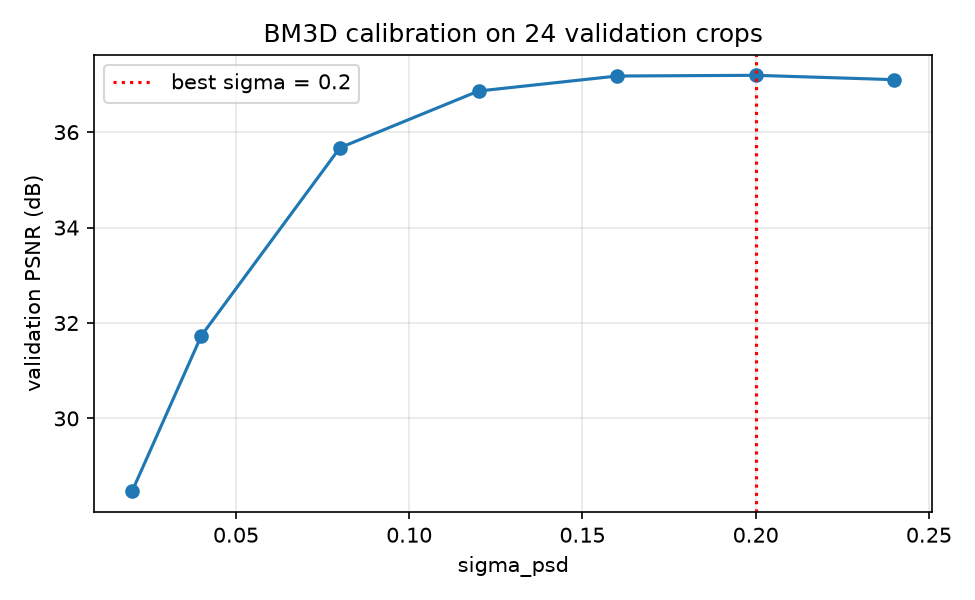
\includegraphics[width=0.60\linewidth]{../../results/figures/calibration.png}
\caption{Validation PSNR against filter strength, measured on 24 validation crops. Both
curves peak inside the grid, BM3D at 0.20 and non-local means at 0.08, so neither result is
limited by where we stopped searching. Non-local means drops off quickly past its peak,
which is the over-smoothing expected once it starts averaging patches that are not really
similar.}
\label{fig:calib}
\end{figure}

\begin{figure}[ht]
\centering
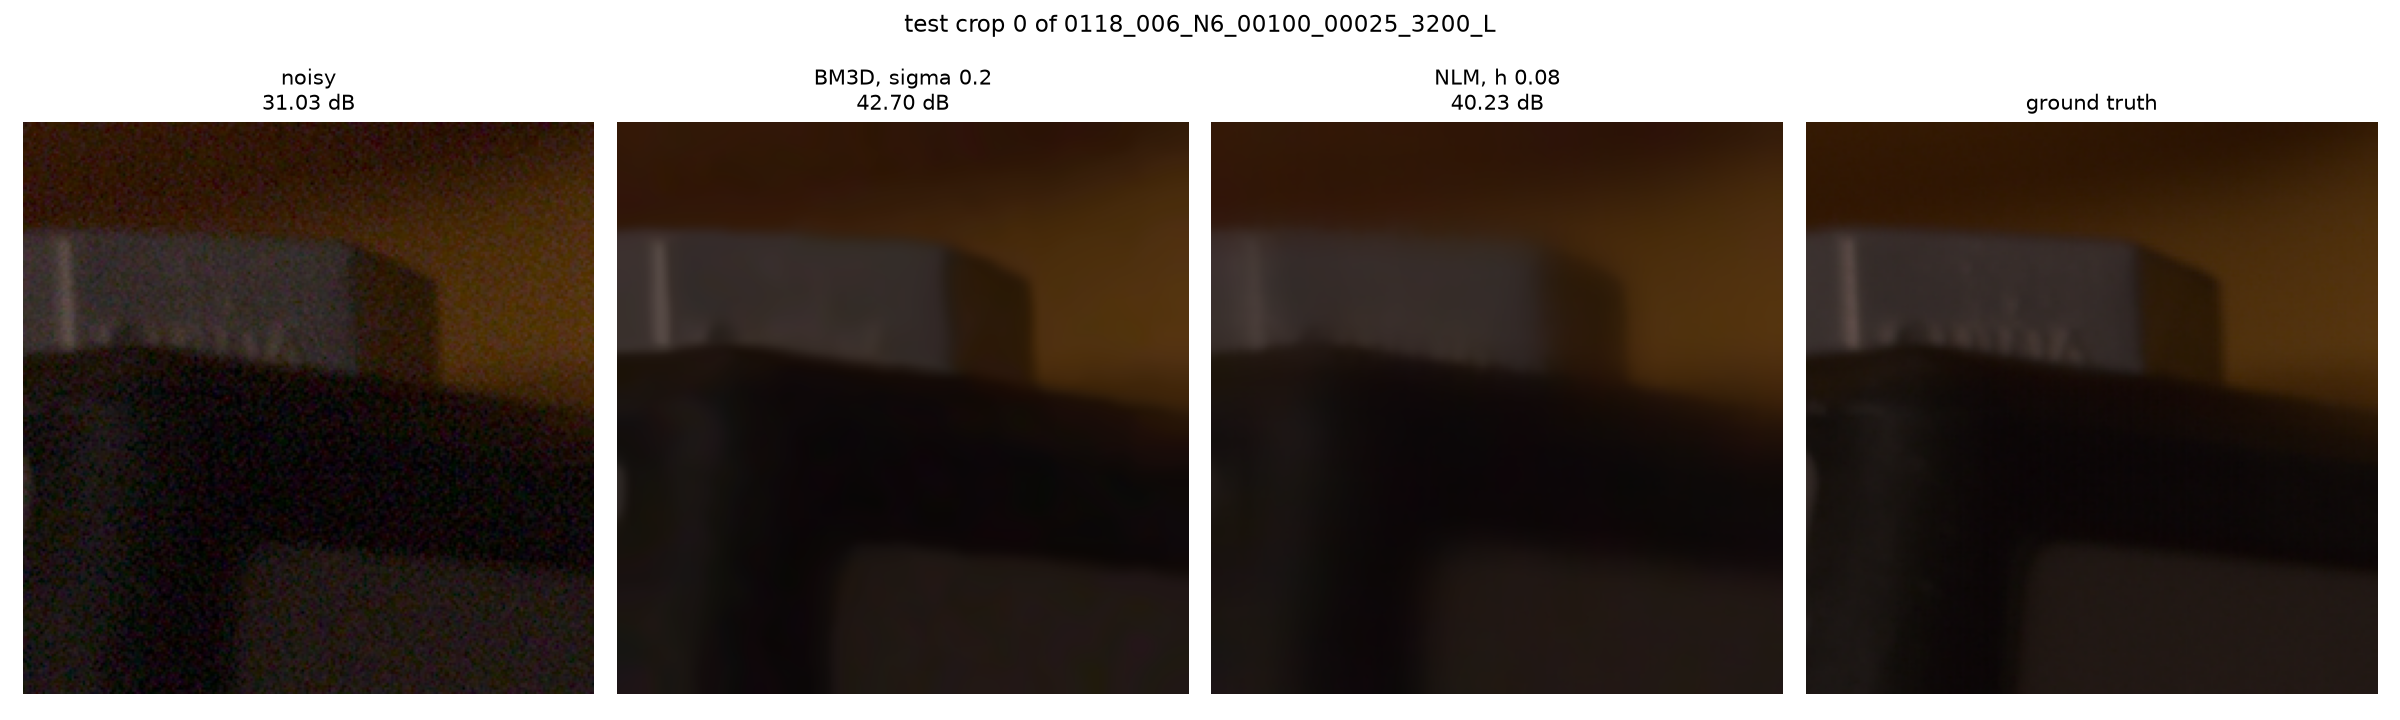
\includegraphics[width=\linewidth]{../../results/figures/qualitative.png}
\caption{One test crop, shot at ISO 100 in low light. BM3D removes the grain while keeping
the lettering on the box readable. Non-local means removes the grain too but blurs the same
detail, which is where its 1.72\,dB deficit comes from.}
\label{fig:qual}
\end{figure}

\section{Proposed Method}
\label{sec:method}
We propose a small Noise2Void denoiser \citep{krull2019noise2void}, trained on the 364
training crops using noisy images only, under the $\mathcal{J}$-invariance framework of
\citet{batson2019noise2self}. We write it ourselves rather than use the authors' package,
because the masking and the loss are the parts of the project we are meant to understand,
and because their released code targets microscopy in a framework we are not using.

\paragraph{The training step.}
The useful property of Noise2Void is that it needs no special architecture. For each
training crop we pick a small random set of pixels $J$, about 2\,\% of the crop, and
overwrite each one with the value of a randomly chosen neighbour. The network sees this
modified crop, and the loss is measured \emph{only} at those pixels, against the original
noisy values:
\begin{equation}
\mathcal{L}(\theta) \;=\; \big\lVert f_\theta(\tilde{y})_J - y_J \big\rVert_2^2 ,
\qquad \tilde{y} = y \text{ with the pixels in } J \text{ replaced}.
\end{equation}
Since the true value at each masked pixel was removed before the network saw it, the
network cannot copy it and has to predict it from the surrounding pixels. Training against
the noisy value still works because the noise has zero mean, so it only adds a constant to
the expected squared error and does not move the minimum
\citep{lehtinen2018noise2noise}. Clean images never enter the loss. We use them only at the
end, to score the result.

\paragraph{The network.}
A plain convolutional network is enough: five $3\times3$ convolution layers with 48
channels and ReLU, then a $1\times1$ layer back to three channels, roughly 90k parameters.
No blind-spot architecture and no U-Net are needed, because the masking already creates the
blind spot. We train with Adam at a learning rate of $10^{-3}$ on random $128\times128$
patches taken from the training crops.

\paragraph{Breaking the spatial correlation.}
Plain Noise2Void assumes the noise is independent from pixel to pixel. This is close enough
to true for the microscopy images it was designed for, but not for our sRGB photos, where
demosaicing and the camera's own denoising spread noise across neighbours
\citep{zhou2020awgn}. Published results show the cost clearly: on the SIDD benchmark plain
Noise2Void reaches only about 27.7\,dB, which is near the level of the noisy input itself.

The established fix is simple to implement. Pixel-shuffle downsampling rearranges the image
into $s^2$ smaller images by taking every $s$-th pixel, which pushes originally adjacent
pixels apart and makes the independence assumption hold much better
\citep{zhou2020awgn}. \citet{lee2022apbsn} used exactly this to take a blind-spot network
from roughly 27.7\,dB to 36.9\,dB on SIDD. We will apply the same step with a stride of
$s = 2$ or $s = 5$, train on the shuffled images, and reassemble the output.

\paragraph{What we will measure.}
Our controlled experiment is the effect of this one design choice: the same network trained
with and without pixel-shuffle downsampling, and at the two stride values, everything else
held fixed. We will also report an untrained control, the average of the allowed
neighbours, because a learned model that cannot beat simple averaging has not learned
anything useful. That control costs nothing and makes a negative result interpretable
rather than confusing.

\section{Feasibility \& Compute Plan}
\label{sec:feasibility}
The compute tier for this project is GPU-light, and all of Milestone 1 in fact ran on the
CPU of an 8-core Windows 11 laptop with 16\,GB of memory. The parameter search took about
15 minutes and scoring the 156 test crops took about 14 minutes, almost all of it BM3D at
5 seconds per crop. Non-local means added about a minute. The dataset is 6.2\,GB on disk
and we load one crop at a time, so memory is never the limit.

The Milestone 2 model is deliberately small. The six-layer network of
Section~\ref{sec:method} has roughly 90k parameters and trains on $128\times128$ patches
cut from the 364 training crops, which is minutes per epoch on a CPU and faster on a basic
GPU. Pixel-shuffle downsampling is a rearrangement of the pixels, so it costs nothing
extra. We are not training a diffusion model. The amount of data is already fixed at 640
crops, 364 of them for training, so no further reduction is needed.

\subsection{Minimum Viable Deliverable (MVP)}
The Noise2Void network of Section~\ref{sec:method} trained on noisy training crops only,
without pixel-shuffle downsampling, scored with the same protocol on the same 156 test
crops and reported next to Table~\ref{tab:baselines}, together with the untrained
neighbour-average control. This is the smallest version that still gives a valid
comparison. We do not expect it to beat BM3D at 38.44\,dB, and the published Noise2Void
result suggests it will not, but a measured result with the reason stated is what the MVP
asks for.

\subsection{Stretch Goal}
If the MVP is working by week 5 or 6 we will add pixel-shuffle downsampling and run the
comparison described in Section~\ref{sec:method}, which is the part we expect to move the
result. After that, and only if time allows, we will train a supervised DnCNN
\citep{zhang2017dncnn} on the paired training crops so our result sits between the
classical and supervised cases, and test the trained model on DND \citep{plotz2017dnd}
without retraining.

\section{Risk Assessment}
\label{sec:risk}
\begin{itemize}[leftmargin=*]
  \item \textbf{The noise is not independent between neighbouring pixels.} Processing inside
  the camera spreads noise across nearby pixels \citep{zhou2020awgn}, so hiding one pixel
  still leaves clues about it in the pixels next to it, and the network can partly learn to
  copy. \citet{cheng2025blindspot} describe the same problem, noting that blind spot
  networks lose local detail because of the independence they assume.
  \emph{What we will do:} this is the known weak point, so we plan for it rather than
  discover it. Pixel-shuffle downsampling is the established fix and is cheap to add. If
  sRGB images stay too difficult even then, SIDD-Small also ships raw images, where the
  noise is much closer to independent.
  \item \textbf{BM3D may simply be better.} At 38.44\,dB it is a strong baseline, and blind
  spot methods often fall short of it on real camera noise.
  \emph{What we will do:} the MVP is defined as a fair comparison, not as a win. We will
  report and explain a negative result rather than tune on the test set until the numbers
  look better.
  \item \textbf{Only two scenes in the test set.} This makes the result less reliable as a
  measure of how the method generalises, and the spread between crops is already large at
  4.39\,dB.
  \emph{What we will do:} report the standard deviation and a per-scene breakdown next to
  the averages, and if time allows rotate which scenes are held out and report how much the
  result moves.
  \item \textbf{The filter settings are only approximately optimal.} They were chosen from
  seven values on 24 crops, so they are close but not provably best.
  \emph{What we will do:} both chosen values sit inside the grid rather than at its edge,
  which is the main thing we needed. Before Milestone 3 we will repeat the search on all
  120 validation crops, which is roughly two hours of CPU time.
  \item \textbf{The DND website is currently down.} We checked it on 1 November 2026 and the
  server returned an error, and the SIDD authors have also moved their own benchmark
  submissions to Kaggle because their evaluation server is offline.
  \emph{What we will do:} DND is only needed for the Milestone 3 generalisation check, not
  for the main comparison, so this does not block us now. If it is still unavailable then,
  we will hold out a third SIDD scene instead and say clearly that the check is on SIDD
  rather than on a second dataset.
\end{itemize}

\section{Work Breakdown}
\label{sec:workbreakdown}
\begin{table}[ht]
\centering
\caption{Who does what, following the task split in the project catalog.}
\label{tab:tasks}
\begin{tabular}{@{}p{0.10\linewidth}p{0.27\linewidth}p{0.27\linewidth}p{0.27\linewidth}@{}}
\toprule
\textbf{Milestone} & \textbf{Student A, data and baseline} & \textbf{Student B, model} & \textbf{Student C, evaluation} \\
\midrule
M1, week 3 & SIDD pipeline, scene split, tuning BM3D and NLM & Design of the noisy-only training objective & PSNR and SSIM protocol, checking the split, results table \\
M2, week 6 & BM3D table on all validation crops & Noise2Void network, first trained model & First comparison against the baseline, figures \\
M3, week 9 & Final classical and, if time allows, supervised baseline & Final model and the hidden-region experiment & Full SIDD and DND comparison, report, demo \\
\bottomrule
\end{tabular}
\end{table}



\section*{Use of AI Tools}
Following course policy, we note that an AI assistant was used to help write and debug the
code in the baseline notebook. All numbers reported here were produced by running
\texttt{notebooks/m1\_baselines.ipynb} in our repository with seed 681 and can be
reproduced from it. 

\bibliographystyle{unsrtnat}
\bibliography{references}

\end{document}
